
\documentclass[11pt]{paper}
\usepackage{graphicx}
\usepackage{epstopdf}
\usepackage{geometry}
\usepackage{caption}
\usepackage{subcaption}
\usepackage{amsmath}
\begin{document}

\title{Work on telegraph neuron model}
\author{Cathal Cooney}
\date{2/7/2014}
\maketitle

In this report a simple model for a neuron is modelled, and the probabilistic background rate is calculated.  Further, the distribution of inter-spike intervals (ISIs) for such a model is calculated, and data is tested to examine for evidence of the model.

\section{Model Process}

The model suggested here is simple, but it is suggested because it is often observed that neurons often find themselves in an up-state (eg. a cone receptor when light is shone into the visual field) or a down-state.

This idea is simplified to the extreme case, where a neuron is either in its up-state and has a high firing-rate, or it is ``off''.   The model is treated as a poisson process, for ease of calculation.

The data that is simulated has an ``up rate'' $\lambda_u$ and a ``down rate'' $\lambda_d$.  For the initial trials, $\lambda_d = 0$.  When in the down-state, the state switches ``up'' with expected frequency $u$, and when in the up-state it switches ``down'' with expected frequency $d$.  Thus, the average background rate, $r$, of the inhomogeneous poisson process can be calculated as:
\begin{equation}\label{lam}
r = \frac{ \frac{\lambda_u }{d}}{ \frac{1}{u} + \frac{1}{d}} = \frac{u\, \lambda_u}{u+d}
\end{equation}
since the expected time for being in the up-state is simply $1/d$ and the expected time in the down-state is $1/u$.

It can be seen then that the expected time for one spike is calculated by letting $r=1$.  This can simplify code, by simply setting 
\begin{equation}
\lambda_u= \frac{u+d}{u}
\end{equation}
and to let the time unit be that of a single expected spike.

\section{Estimating the firing rate $r(t)$}

With the model for the firing rate as above, it is possible to explicitly calculate the probability of being in the up-state for the time following a spike.  In the initial setting, where $\lambda_d$ is set to zero, then it is known when there is a spike that the rate is in the up-state, so at the time of spiking $t_0$ the probability $p(t_0)$ of being in the up-state is equal to one.  For the estimate of the rate, $\tilde{r}(t)$, this is reflected by setting $\tilde{r}(t_0) = \lambda_u$.  Then, the probability is reset every time there is a spike, so it is only required to calculate the probability of being in the up-state given that there has been no spike since the time $t_0$ of the last spike.  Using Baye's Theorem it is possible to calculate the probability of being in the up-state at a time $t+\Delta t$, given a spike at time $t=t_0$ for small $\Delta t$.

Let $X=$ up at $t=t_0+\Delta t$, $Y=$ no spike since $t=t_0$ and $Z=$ spike at $t=t_0$. Then,
\begin{equation}\label{p}
P(X|Y|Z) = \frac{P(Y|X|Z)P(X|Z)}{P(Y|Z)} = \frac{(1-\lambda_u \Delta t) (1-d \Delta t)}{1-r\Delta t}
\end{equation}

Then, it is possible to calculate the first approximation to the probability  of being up at time $t$, by letting $t_0=0, \,\Delta t =t/n$.

\begin{equation}
\begin{split}
P(\mbox{up at } t | Y | Z)   &=  \lim_{n \rightarrow \infty}\prod_{k=1}^n \frac{(1-\lambda_ut/n)(1-dt/n)}{1-rt/n}  \\
&= \lim_{n \rightarrow \infty} \prod_{k=1}^n \left(1+ t\frac{r-\lambda_u-d}{n}\right) \\
& = \lim_{n \rightarrow \infty} \left(1 + t\frac{r-\lambda_u -d}{n} \right)^n \\
&=  e^{(r-\lambda_u-d)t}
\end{split}
\end{equation}

Recalling from equation \ref{lam} that $\lambda_u = r(u+d)/u$, get:
\begin{equation}
p=e^{-\frac{d(r+u)}{u}(t-t_0)}
\end{equation}

Comparing this to the exponential kernel in the Van Rossum metric \cite{vanRossum2001}, then:
\begin{equation}
\tau = \frac{u}{d(r+u)}
\end{equation}

This is clearly just the first approximation, since it does not take into account the possibility of the model switching into the down-state and back up.  To calculate the full probability, let $y(t) = P(\mbox{up at } t | Y | Z)$, with $Y,Z$ as in equation \ref{p} above.  Then:

\begin{equation}
\begin{split}
y(t+h) &=  y(t)P(\mbox{staying in up-state} | \mbox{up at t}|Y|Z)  \\
& + (1-y(t))P(\mbox{switching up} | \mbox{down at t}|Y|Z)\\
&\\
&= y(t)\left( \frac{(1-dh)(1-\lambda_uh)}{1-rh} \right) + (1-y(t)) \left(\frac{(uh)(1)}{1-rh}  \right)\\
&\\
& = y(t)\left( 1 + h(r-d-\lambda_u-u ) \right) + uh
\end{split}
\end{equation}

\begin{figure}[b!]
\begin{center}
\resizebox{0.75\textwidth}{!}{% GNUPLOT: LaTeX picture with Postscript
\begingroup
  \makeatletter
  \providecommand\color[2][]{%
    \GenericError{(gnuplot) \space\space\space\@spaces}{%
      Package color not loaded in conjunction with
      terminal option `colourtext'%
    }{See the gnuplot documentation for explanation.%
    }{Either use 'blacktext' in gnuplot or load the package
      color.sty in LaTeX.}%
    \renewcommand\color[2][]{}%
  }%
  \providecommand\includegraphics[2][]{%
    \GenericError{(gnuplot) \space\space\space\@spaces}{%
      Package graphicx or graphics not loaded%
    }{See the gnuplot documentation for explanation.%
    }{The gnuplot epslatex terminal needs graphicx.sty or graphics.sty.}%
    \renewcommand\includegraphics[2][]{}%
  }%
  \providecommand\rotatebox[2]{#2}%
  \@ifundefined{ifGPcolor}{%
    \newif\ifGPcolor
    \GPcolorfalse
  }{}%
  \@ifundefined{ifGPblacktext}{%
    \newif\ifGPblacktext
    \GPblacktexttrue
  }{}%
  % define a \g@addto@macro without @ in the name:
  \let\gplgaddtomacro\g@addto@macro
  % define empty templates for all commands taking text:
  \gdef\gplbacktext{}%
  \gdef\gplfronttext{}%
  \makeatother
  \ifGPblacktext
    % no textcolor at all
    \def\colorrgb#1{}%
    \def\colorgray#1{}%
  \else
    % gray or color?
    \ifGPcolor
      \def\colorrgb#1{\color[rgb]{#1}}%
      \def\colorgray#1{\color[gray]{#1}}%
      \expandafter\def\csname LTw\endcsname{\color{white}}%
      \expandafter\def\csname LTb\endcsname{\color{black}}%
      \expandafter\def\csname LTa\endcsname{\color{black}}%
      \expandafter\def\csname LT0\endcsname{\color[rgb]{1,0,0}}%
      \expandafter\def\csname LT1\endcsname{\color[rgb]{0,1,0}}%
      \expandafter\def\csname LT2\endcsname{\color[rgb]{0,0,1}}%
      \expandafter\def\csname LT3\endcsname{\color[rgb]{1,0,1}}%
      \expandafter\def\csname LT4\endcsname{\color[rgb]{0,1,1}}%
      \expandafter\def\csname LT5\endcsname{\color[rgb]{1,1,0}}%
      \expandafter\def\csname LT6\endcsname{\color[rgb]{0,0,0}}%
      \expandafter\def\csname LT7\endcsname{\color[rgb]{1,0.3,0}}%
      \expandafter\def\csname LT8\endcsname{\color[rgb]{0.5,0.5,0.5}}%
    \else
      % gray
      \def\colorrgb#1{\color{black}}%
      \def\colorgray#1{\color[gray]{#1}}%
      \expandafter\def\csname LTw\endcsname{\color{white}}%
      \expandafter\def\csname LTb\endcsname{\color{black}}%
      \expandafter\def\csname LTa\endcsname{\color{black}}%
      \expandafter\def\csname LT0\endcsname{\color{black}}%
      \expandafter\def\csname LT1\endcsname{\color{black}}%
      \expandafter\def\csname LT2\endcsname{\color{black}}%
      \expandafter\def\csname LT3\endcsname{\color{black}}%
      \expandafter\def\csname LT4\endcsname{\color{black}}%
      \expandafter\def\csname LT5\endcsname{\color{black}}%
      \expandafter\def\csname LT6\endcsname{\color{black}}%
      \expandafter\def\csname LT7\endcsname{\color{black}}%
      \expandafter\def\csname LT8\endcsname{\color{black}}%
    \fi
  \fi
  \setlength{\unitlength}{0.0500bp}%
  \begin{picture}(7200.00,5040.00)%
    \gplgaddtomacro\gplbacktext{%
      \csname LTb\endcsname%
      \put(946,503){\makebox(0,0)[r]{\strut{} 0.3}}%
      \put(946,1113){\makebox(0,0)[r]{\strut{} 0.4}}%
      \put(946,1724){\makebox(0,0)[r]{\strut{} 0.5}}%
      \put(946,2334){\makebox(0,0)[r]{\strut{} 0.6}}%
      \put(946,2944){\makebox(0,0)[r]{\strut{} 0.7}}%
      \put(946,3554){\makebox(0,0)[r]{\strut{} 0.8}}%
      \put(946,4165){\makebox(0,0)[r]{\strut{} 0.9}}%
      \put(946,4775){\makebox(0,0)[r]{\strut{} 1}}%
      \put(1078,220){\makebox(0,0){\strut{} 0}}%
      \put(1651,220){\makebox(0,0){\strut{} 1.0}}%
      \put(2223,220){\makebox(0,0){\strut{} 2.0}}%
      \put(2796,220){\makebox(0,0){\strut{} 3.0}}%
      \put(3368,220){\makebox(0,0){\strut{} 4.0}}%
      \put(3941,220){\makebox(0,0){\strut{} 5.0}}%
      \put(4513,220){\makebox(0,0){\strut{} 6.0}}%
      \put(5086,220){\makebox(0,0){\strut{} 7.0}}%
      \put(5658,220){\makebox(0,0){\strut{} 8.0}}%
      \put(6231,220){\makebox(0,0){\strut{} 9.0}}%
      \put(6803,220){\makebox(0,0){\strut{} 10.0}}%
      \put(176,2639){\makebox(0,0){\strut{}$\tau/\tau_{o}$}}%
      \put(3900,0){\makebox(0,0){\strut{} $u$}}%
    }%
    \gplgaddtomacro\gplfronttext{%
    }%
    \gplbacktext
    \put(0,0){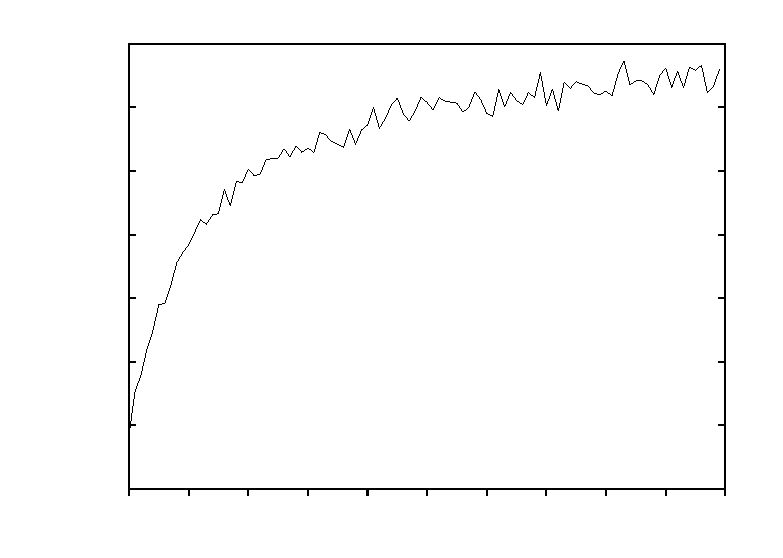
\includegraphics{tauoptoverpred}}%
    \gplfronttext
  \end{picture}%
\endgroup
}
\caption{\label{predovertauopt} This figure shows the ratio of the predicted value for $\tau$ in an exponential model over the empirical optimised value $\tau_o$.}
\end{center}
\end{figure}

This leads to the following ordinary differential equation:

\begin{equation}
y^\prime(t) = \left( r - d - u - \lambda_u \right)y(t) + u
\end{equation}

This ODE has general solution:
\begin{equation}
y(t) = Ce^{(r-d-u-\lambda_u)(t-t_0)} + \frac{u}{u+d+\lambda_u - r}
\end{equation}

Since $y(t_0) = 1$, get:
\begin{equation}
y(t) = \frac{d+\lambda_u - r}{d+u+\lambda_u -r} e^{(r-d-u-\lambda_u)(t-t_0)} + \frac{u}{u+d+\lambda_u-r}
\end{equation}

Letting $\lambda_u = r(u+d)/u$, get:
\begin{equation}
y(t) = \frac{d(u+r)}{u^2 + d(u+r)} e^{-\frac{u^2+d(u+r)}{u}(t-t_0)} + \frac{u^2}{u^2+ d(u+r)}
\end{equation}

This solution was tested against a standard exponential model, which was minimised over $\tau$ with a downhill simplex method.  Figure \ref{predovertauopt} shows how the ratio of the predicted value for $\tau$ over the optimised value rises towards one as the value for $u$ increases.  This suggests that, while this method is clearly not completely correct, that it is at least a reasonable approximation.

\section{Markov Process}

The switching of the up and down states defines a Continuous-time Markov Chain (CTMC).  That is, the future of the process does not depend on the past at all, merely whether the model is currently in the up-state or the down-state.

By the theory of Markov Chains, this process can be described by the simultaneous differential equations:
\begin{equation}
\left\{
\begin{split} &p_u^{\prime}(t) = -dp_u(t) + dp_d(t)\\ &p_d^{\prime}(t)=up_u(t) - up_d(t)
\end{split}
\right.
\end{equation}
This is simply the linear ODE:
\begin{equation}
P^{\prime}(t) = P(t)Q
\end{equation}
where
\begin{equation}
Q =  \begin{pmatrix} -d & d \\ u & -u \end{pmatrix}
\end{equation}

Then the solution to the matrix $P(t)$ is simply the exponential, $e^{tQ}$ of the transition matrix $Q$. 

\begin{equation}
P(t) = e^{tQ} = \begin{pmatrix} \frac{u}{u+d}+\frac{d}{u+d}e^{-(u+d)t} & \frac{d}{u+d} - \frac{d}{u+d}e^{-(u+d)t} \\ \frac{u}{u+d} - \frac{u}{u+d}e^{-(u+d)t} & \frac{d}{u+d} + \frac{u}{u+d}e^{-(u+d)t}\end{pmatrix}
\end{equation}


To calculate the probability of being in the up-state at a time $t$ after a spike at $t=0$, provided there has been no spike since $t=0$, it suffices to calculate the exponential of the transition matrix $Q_s$ below:

\begin{equation}
Q_s = \begin{pmatrix} -d-\lambda_u & d & \lambda_u \\ u & -u & 0 \\ 0 & 0 & 0\end{pmatrix}
\end{equation}

The third state of the Markov chain described by the transition matrix $Q_s$ is an ``absorbing'' state, the state of spiking, from which it is impossible to return to either the up or the down state.

The solution to the spiking Markov chain is:
\begin{equation}
P(t)  = \begin{pmatrix} Ae^{-\alpha t} + (1-A)e^{-\beta t} & Be^{-\alpha t} - Be^{-\beta t} & 1 - (A+B)e^{-\alpha t} - (1-A-B)e^{-\beta t} \\ Ce^{-\alpha t} - Ce^{-\beta t} & (1-A)e^{-\alpha t} +  Ae^{-\beta t} & 1 - (1-A+C)e^{-\alpha t} - (A+C)e^{-\beta t} \\ 0 & 0 & 1 \end{pmatrix}
\end{equation}
where $-\alpha,-\beta$ are the roots to the characteristic polynomial of $Q_s$.
\begin{equation}
\begin{split}
-\alpha = \frac{-(u+d+\lambda_u) + \sqrt{(u-d-\lambda_u)^2 + 4ud}}{2}\\
-\beta = \frac{-(u+d+\lambda_u) - \sqrt{(u-d-\lambda_u)^2 + 4ud}}{2}
\end{split}
\end{equation}
Since $u,d,\lambda_u >0$, these probabilities are simply double exponentials, and there are no trigonometric terms.

Specifically:
\begin{equation}
\begin{split}
&A = \frac{\left(u-d-\lambda_u+\sqrt{(u-d-\lambda_u)^2+4ud}\right)}{2\sqrt{(u-d-\lambda_u)^2+4ud}}\\
&B = \frac{d}{\sqrt{(u-d-\lambda_u)^2+4ud}}\\
&C = \frac{u}{\sqrt{(u-d-\lambda_u)^2+4ud}}
\end{split}
\end{equation}
It can be  easily confirmed that $A,B,C>0$, which is necessary to ensure that all the probabilities are between 0 and 1.

If the model is changed such that there is a non-zero spiking probability, $\lambda_d>0$, in the down-state, then the transition matrix $Q_s$ becomes:
\begin{equation}
Q_s = \begin{pmatrix} -d-\lambda_u & d & \lambda_u \\ u & -u-\lambda_d & \lambda_d \\ 0 & 0 & 0 \end{pmatrix}
\end{equation}

This matrix has solution:
\begin{equation}
\begin{pmatrix}
Ae^{-\alpha t} + (1-A)e^{-\beta t} & B\left(e^{-\alpha t} - e^{-\beta t}\right) & 1-e^{-\beta t} - (A+B)\left(e^{-\alpha t} - e^{-\beta t}\right) \\
C\left(e^{-\alpha t} - e^{-\beta t}\right) & (1-A)e^{-\alpha t} + Ae^{-\beta t} & 1-e^{-\alpha t} - (C-A)\left(e^{-\alpha t} - e^{-\beta t}\right)\\
0 & 0 & 1
\end{pmatrix}
\end{equation}
where $-\alpha,-\beta$ are once again the roots of the characteristic polynomial of $Q_s$.
\begin{equation}
\begin{split}
-\alpha = \frac{-(u+d+\lambda_u+\lambda_d) + \sqrt{(u-d+\lambda_d-\lambda_u)^2+4ud}}{2}\\
-\beta = \frac{-(u+d+\lambda_u+\lambda_d) - \sqrt{(u-d+\lambda_d-\lambda_u)^2+4ud}}{2}
\end{split}
\end{equation}
again, $u,d>0$ means that the probabilities above are all double exponentials, with no trigonometric terms.

\begin{equation}
\begin{split}
& A = \frac{u-d+\lambda_d-\lambda_u + \sqrt{(u-d+\lambda_d-\lambda_u)^2+4ud}}{2\sqrt{(u-d+\lambda_d-\lambda_u)^2 + 4ud}}\\
& B = \frac{d}{\sqrt{(u-d+\lambda_d-\lambda_u)^2 + 4ud}}\\
& C = \frac{u}{\sqrt{(u-d+\lambda_d-\lambda_u)^2 + 4ud}}
\end{split}
\end{equation}

To simplify notation, set:
\begin{equation}
\begin{split}
\label{dg}
\Delta &= \lambda_u - \lambda_d\\
\gamma &= \sqrt{(u-d-\Delta)^2 + 4ud}
\end{split}
\end{equation}

Thus:
\begin{equation}
\begin{split}
A = \frac{u-d - \Delta + \gamma}{2\gamma},\, B = \frac{d}{\gamma}, \,C = \frac{u}{\gamma}
\end{split}
\end{equation}

\subsection{Estimating the rate function $r(t)$}

These probabilities can now be used to calculate the estimated rate function, $r(t)$, based on the timing of spikes.  Assuming that the probability of the last spike is known, then the rate function between any two spikes is estimated by this Markov model. 

If the probability vector at the time of the last spike is ${\bf p_0}=(p_0, 1-p_0,0)$, then the probabilities at a time $t$ after the spike are:
\begin{equation}
{\bf p(t)} = {\bf p_0}e^{Q_s} = (p_u(t),p_d(t),p_s(t))
\end{equation}
where
\begin{equation}
\begin{split}
p_u(t) &= (p_0(A-C)+C)e^{-\alpha t}+(p_0(1-A+C)-C)e^{-\beta t}\\
p_d(t) &= (p_0(A+B-1)+1-A)e^{-\alpha t}+(p_0(-A-B)+A)e^{-\beta t}\\
p_s(t) &= 1 - p_u(t) - p_d(t)
\end{split}
\end{equation}

The probabilities $p_u(t), \,p_d(t)$ represent the probability of being in the up/down state and not spiking.  The probability required to calculate the rate function, $r(t)$, between spikes is the probability of being in the up-state given that there has not been a spike.  This is because it is known that there has been no spike since the last spike.  Therefore, by Baye's Theorem, the probability $p(t)$ is just:
\begin{equation}
p(t)  = \frac{p_u(t)}{p_u(t) + p_d(t)}
\end{equation}
so, the rate function becomes:
\begin{equation}
r(t) = \Delta p(t) + \lambda_d = \frac{A_0e^{-\alpha t}+B_0e^{-\beta t}}{C_0e^{-\alpha t} + D_0e^{\beta t}}
\end{equation}
where:
\begin{equation}
\begin{split}
\label{abcd}
A_0 & = \Delta(p_0(-u-d-\Delta + \gamma)+2u)+\lambda_d(p_0(-2\Delta)+u+d+\Delta+\gamma)\\
B_0 & =\Delta(p_0(u+d+\Delta + \gamma)-2u)+\lambda_d(p_0(2\Delta)-u-d-\Delta+\gamma)\\
C_0 & = p_0(-2\Delta)+u+d+\Delta+\gamma\\
D_0 & = p_0(2\Delta) -u-d-\Delta + \gamma
\end{split}
\end{equation}

\subsection{Change in probability when a spike arrives}

In the previous section, the rate function, $r(t)$, and the pdf of the ISI distribution, $p_{ISI}(t)$, were calculated, given that the probability of being in the up-state at the time of the last spike, $p_0$, is known.  However, it is necessary to reevaluate the probability at the time a spike arrives.

If the probability of being in the up-state before the spike is $p_u(t)$, then the presence of a spike provides information on the state of the model. By Baye's Theorem:

\begin{equation}
\begin{split}
P(\mbox{up-state} | \mbox{spike}) &= \frac{P(\mbox{spike}|\mbox{up-state})P(\mbox{up-state})}{P(\mbox{spike})} \\
&=\frac{\lambda_u p_u(t)}{\Delta p_u(t) + \lambda_d }
\end{split}
\end{equation}

Thus:
\begin{equation}
p_u(t) \rightarrow \frac{\lambda_u p_u(t)}{\Delta p(t) + \lambda_d}
\end{equation}

equivalently:
\begin{equation}
\begin{split}
r(t) \rightarrow &(\lambda_u - \lambda_d)\frac{\lambda_u p_u(t)}{\Delta p_u(t)+ \lambda_d} + \lambda_d\\
= &\frac{\lambda_u^2 p_u(t) - \lambda_u\lambda_dp_u(t)+\lambda_u\lambda_dp_u(t) + \lambda_d^2(1-p_u(t))}{\lambda_u p_u(t) + \lambda_d(1- p_u(t))}\\
= & \frac{\lambda_u^2 p_u(t) + \lambda_d^2(1-p_u(t))}{\lambda_up_u(t) + \lambda_d(1-p_u(t))}
\end{split}
\end{equation}

\subsection{Calculating the ISI distribution from the estimated rate function}
When dealing with spike-train data, it is very useful to know the inter-spike interval (ISI) distribution, as this can be observed much easier than the firing rate of a neuron.

The ISI distribution for an inhomogeneous Poisson process, with rate function $r(t)$, is:
\begin{equation}
p_{ISI}(t) = r(t) e^{-\int_0^t r(s)\,ds}
\end{equation}

Now it is necessary to integrate the rate function from $0$ to $t$:
\begin{equation}
\begin{split}
\label{int}
\int_0^t r(s)\,ds &= \int_0^t  \frac{A_0e^{-\alpha s}+B_0e^{-\beta s}}{C_0e^{-\alpha s} + D_0e^{\beta s}}\,ds\\ 
&= \frac{\alpha A_0D_0 - \beta B_0 C_0}{(\alpha - \beta)C_0D_0}t + \frac{B_0 C_0-A_0D_0}{(\alpha - \beta)C_0D_0} \log\left({\frac{C_0e^{\beta t} + D_0e^{\alpha t}}{C_0 + D_0} }\right)
\end{split}
\end{equation}

Substituting equations \ref{abcd} and \ref{dg}, and noting that $\beta-\alpha=\gamma$, the fractions in the above equation become:
\begin{equation}
\begin{split}
\frac{\alpha A_0D_0 - \beta B_0 C_0}{(\alpha - \beta)C_0D_0} &= u+d+\lambda_u+\lambda_d = \alpha+\beta,\\
 \frac{B_0 C_0-A_0D_0}{(\alpha - \beta)C_0D_0} &= -1
\end{split}
\end{equation}
Thus equation \ref{int} becomes:
\begin{equation}
\begin{split}
\int_0^t r(s)\,ds &= (\alpha+\beta)t - \log\left( {\frac{C_0e^{\beta t} + D_0e^{\alpha t}}{C_0 + D_0} }\right) \\
&= \log\left( e^{(\alpha+\beta)t}\right) + \log \left( \frac{C_0 +D_0}{C_0e^{\beta t}+ D_0e^{\alpha t}}\right)\\
&= \log \left( \frac{C_0e^{(\alpha+\beta)t}+D_0e^{(\alpha+\beta)t}}{C_0e^{\beta t}+D_0e^{\alpha t}}\right)\\
&= \log \left( \frac{C_0+D_0}{C_0e^{-\alpha t}+D_0e^{-\beta t}}\right)
\end{split}
\end{equation}

Now $p_{ISI}(t)$ becomes:
\begin{equation}
\begin{split}
p_{ISI}(t) &= \frac{A_0e^{-\alpha t}+B_0e^{-\beta t}}{C_0e^{-\alpha t} + D_0e^{-\beta t}}e^{-\log \left( \frac{C_0+D_0}{C_0e^{-\alpha t}+D_0e^{-\beta t}}\right)}\\
& = \frac{A_0e^{-\alpha t}+B_0e^{-\beta t}}{C_0e^{-\alpha t} + D_0e^{-\beta t}}e^{\log \left( \frac{C_0e^{-\alpha t}+D_0e^{-\beta t}}{C_0+D_0}\right)}\\
&= \frac{A_0e^{-\alpha t}+B_0e^{-\beta t}}{C_0e^{-\alpha t} + D_0e^{-\beta t}}\left( \frac{C_0e^{-\alpha t}+D_0e^{-\beta t}}{C_0+D_0}\right)\\
&= \frac{A_0}{C_0+D_0}e^{-\alpha t} + \frac{B_0}{C_0+D_0}e^{-\beta t}
\end{split}
\end{equation}

This is the probability density function (pdf) of a bimodal hyper-exponential distribution.

\section{Testing on data}
The previous result allows for testing on real data.  The data used in this report is the data used in the paper by Sen et al. \cite{} on kernel density estimation as a tool 



\end{document}
